\documentclass[11pt]{amsart}

% Standard letter size paper with 1inch margins
\usepackage[letterpaper, margin=1in]{geometry}

% Useful packages 
\usepackage{amsmath, amssymb, amsthm, amsaddr}
\usepackage{enumerate, subcaption, graphicx, hyperref, float}


\title{AMATH 482/582: Homework 4}
\author{Jonathan McCormack}
\address{Applied Mathematics Department, University of Washington, Seattle, WA 
\\jrmack20@uw.edu}
\date{\today}

\begin{document}



\begin{abstract}
    Wine can be chemically analyzed to produce rich data that can be assesed by supervised machine 
    learning algorithms to predict which wine will be ranked the best by wine experts. The data 
    measures 11 chemical 'features' and outputs a score from 0 (low) to 10 (high) for each wine 
    sample. Supervised learning based on linear regression and kernal ridge regression is well suited 
    for evaluating and ranking samples based on their features. We also used one-hot encoding and 
    k-fold cross validation to improve the unbiased, predictive power of the model. We discovered a 
    limited, linear correlation between the chemical features and how the wine was scored.

\end{abstract}

\maketitle 

\section{Introduction and Overview}\label{sec:Introduction}

Machine learning provides a powerful framework for extracting meaningful insights from complex datasets 
by evaluating the intricate relationships between input features and target outputs. In particular, 
supervised machine learning has found extensive real-world applications because it leverages validated, 
historical information to train predictive models. By utilizing datasets where the ground truth is already 
known, we can build models that reasonably predict outputs for new, unseen data based on established patterns 
in the input features. \\

In this study, we apply these principles to the physicochemical analysis of wine to develop an algorithm 
capable of predicting quality scores. We compare the efficacy of linear regression, Gaussian kernel ridge regression, 
Laplacian kernel ridge regression, and Polynomial kernel ridge regression to determine which mathematical 
approach best captures the trends within the Portuguese "Vinho Verde" dataset.

\section{Theoretical Background}\label{sec:Theory}

In supervised learning, we are given a data set of n input-output pairs ${(x_i,y_i)}_{i=1}^n$, and we assume the data 
is goverend by a unknown, underlying function\eqref{equ:true-func} corrupted by additive noise. This noise is assumed to be independent and 
identically distributed gaussian ($\epsilon_i \sim N(0, \sigma^2)$). Thus, the goal of supervised learning is to find 
some $\hat{f}(x)$ that estimates the true, underlying function $f^\dagger(x)$. To achieve this, we 'fit' the known input-output 
data to different model classes $\mathcal{F}$, such as linear, gaussian, laplacian, polynomial, etc.

\begin{equation}
    y_i = f^\dagger(x_i) + \varepsilon_i
    \label{equ:true-func}
\end{equation}

\subsection{Data pre-processing and One-hot encoding}\label{sec:One-hot-encoding}

In this case, the input data is a matrix where each row is a different wine sample and each column is a different chemical feature. 
Since different features are measured with different scales and units, the feature data must be normalized to ensure the model does not 
over or undervalue certain features because their measurement is larger or smaller. The data is normalized by subtracting the mean 
of each feature and dividing by the standard deviation of the feature. Because the output of this problem are discrete groups of wine quality 
rather than some scalar metric, this problem is classification and not simply regression. This means two things: the output scores must 
be separated during pre-processing and the output of the function must be separated before reporting. One-hot encoding is used because there 
are multiple possible output scores; this is done by transforming the given output vector into an output array where each row is still a sample, but 
the columns are all zero except a one in the column that represents that sample's group. For example: an output score of [3] would be transformed 
to an output of [0, 0, 0, 1, 0, 0, 0, 0, 0, 0, 0]. After a model is created and applied to a new set of data, the output of the model will be a 
similar matrix and each sample's score will be the column with the highest value representing the most similar group to that sample.\\

\subsection{Linear Regression}\label{sec:Linear}

The simplest way to model the relationship between these features is to use linear regression. Linear regression assumes that 
the features are linearly related (in the linear model class $\mathcal{F}$), with some features having more weight than other features 
in determining the output quality score. The linear model class produces functions of the form 
$\hat{f}(\underline{x}) = \theta_0 + \theta_1 x_1 + \dots + \theta_n x_n + \epsilon$, where $\theta_0$ is the intercept point and the 
remaining $\theta$ values are the coefficients for each feature. We consider the data to exist in 
$\mathbb{R}^{n+1}$ space for n number of features. The solution is an array of $\theta$ vectors, where each column vector is the coefficients 
to a linear hyperplane that best represents that respective column of outputs\cite{stranglinalg}. That hyperplane will not intersect all datapoints in its group, 
but will minimize the error (distance) of any point in that group from the appropriate hyperplane for that group. Since the $\theta$ vector 
is the coefficients of the linear model, we can calculate the inner product of [1, $x_i^T$] and a $\theta$ vector to calculate the projection of
$x_i$ onto that output classes' hyperplane. Since the error is the difference between the true value, $y_i$, and the approximate value, 
[1, $x_i^T$]$\theta$, we can minimize the error by solving the below optimization problem\eqref{equ:linear-optimization-problem}. This problem 
minimizes the Mean Squared Error (MSE) of any data point from its group's hyperplane. An important note is that because of 
one-hot encoding, the true output score should be zero in all but one column for every row; this is how each sample in the training data helps 
build not only the function for its group, but also the function for all groups it does not occupy.

\begin{equation}
    \hat{\theta} = \arg\min_{\theta} \frac{1}{m} \sum_{i=1}^{m} \| \boldsymbol{Y} - \boldsymbol{X}\boldsymbol\theta \|^2_2
    \label{equ:linear-optimization-problem}
\end{equation}

The solution to the above optimization problem is found using the normal equations as in the below equation\eqref{equ:linear-solution} 
by understanding that the error vector must be orthogonal to (in the Nullspace of) the transpose of the data matrix\cite{stranglinalg}. 
This makes sense because the lowest error is perpendicular to the hyperplane. 

\begin{equation}
    \begin{split}
        X^T(Y - X\hat{\theta}) = 0\\
        \hat{\theta} = (X^TX)^{-1} X^TY
    \end{split}
    \label{equ:linear-solution}
\end{equation}

\subsection{Regularization and Cross-Validation}\label{sec:Regularization}

When developing a model for a set of data, regardless of the model classes $\mathcal{F}$, if we overfit the data by mimizing the error on the training data, 
we may lower the training MSE, but increase the validation test MSE leading to a poor model for future predictions. An overfit model is considered to have 
low bias because it has lowered $\text{Bias}^2[\hat{f}(x)] = \left( \mathbb{E}[\hat{f}(x)] - f(x) \right)^2$. The high error in an overfit model is called 
variance, where $\text{Var}[\hat{f}(x)] = \mathbb{E}\left[ \left( \hat{f}(x) - \mathbb{E}[\hat{f}(x)] \right)^2 \right]$. We can balance the bias and variance 
error by applying regularization, where we add a regularization parameter that penalizes a function for having too heavily weighted coefficients (which would 
otherwise ensure all data, including noise, would be included in the model). The optimization problem in the regularization case is listed below\eqref{equ:regularization-optimization-problem}. 
Ridge regression (Tikhonov regularization) uses the squared $L_2$ norm of the coefficient vector ($\hat{\theta}$) as a penalty term in the loss function. 
Regularization is scaled with $\lambda$ (scikit-learn uses $\alpha$), where a low value of $\lambda$ has little regularization (potentially overfit) and a 
high $\lambda$ has strong regularization (potentially underfit). We adjust the value of the $\lambda$ parameter until we lower the total MSE when the model 
is applied to the validation test data. Similarly to the ordinary least squares problem, we can solve the regularized regression problem using the normal equations 
as in the below quation\eqref{equ:ridge-regression-solution}.\\


\begin{equation}
    \hat{\theta} = \arg\min_{\theta} \frac{1}{m} \sum_{i=1}^{m} \| \boldsymbol{Y} - \boldsymbol{X}\boldsymbol\theta \|^2_2+ \lambda \|\theta\|_2^2
    \label{equ:regularization-optimization-problem}
\end{equation}

\begin{equation}
    \hat{\theta_\lambda} = (A^TA + \lambda I)^{-1}A^Ty_{train}
    \label{equ:ridge-regression-solution}
\end{equation}

In order to find the best value of the regularization parameters, we apply cross validation, the technique of training the model on a subset of the training data and 
using the remaining data to score the regularization parameter. The key benefit is that in the end, the model was not trained on the validation test data, this means 
the validation MSE is a true measure of the model's efficacy, because the model wasn not exposed to that test data set in training. We used k-fold cross validation, 
where we set a number of folds, k, and randomly sort the training data into those k folds. We train the data on all but one fold and test the data on the remaining data. 
This process is repeated k times and the score is averaged. This process is repeated for every combination of the parameters, which is especially useful in more complex 
models. This allows us to isolate the best combination of parameters to lower both sources of reducible error, bias and variance.

\subsection{Kernel Methods}\label{sec:Kernel-Methods}

In rare cases will a data set have a clear, linear relationship between the input features and the output scores, 
real-world data often includes non-linear interactions that ordinary least squares regression does not account for. 
This is made especially difficult because computing all possible nonlinear interactions is incredibly costly with large samples of high 
dimensional data. The Kernel Ridge Regrssion (KRR) method allows us to bypass some of these computations by using unique properties of 
Reproducing Kernel Hilbert Spaces. Simply put, the Kernel calculates the inner product of every possible combination of the data vectors by 
applying some kernel function. This allows nonlinear functions to be applied to vectors. This also allows us to see which vectors are related or disimilar. 
Ultimately, it converts a nonlinear optimization problem into the below linear optimization problem\eqref{equ:krr-optimization-problem}. 

\begin{equation}
    \begin{split}
        f(x_i) = \sum_{j=1}^{n} \alpha_j K(x_i, x_j)\\
        \hat{\alpha} = \arg\min_{\alpha} \|\mathbf{Y} - K\alpha\|_2^2 + \lambda \alpha^\top K \alpha
    \end{split}
    \label{equ:krr-optimization-problem}
\end{equation}

By expanding the norm term and finding the gradient of the loss function, we can find the optimal $\alpha$ vector by solving the below equation\eqref{equ:krr-solution}.

\begin{equation}
    \alpha = (K + \lambda I)^{-1}\mathbf{Y}
    \label{equ:krr-solution}
\end{equation}

Cross validation for KRR uses more hyperparameters that ordinary least squares regression. We still use the regularization scaling coefficient 
$\lambda$ (scikit-learn uses $\alpha$). When using the Gaussian/Radial Basis Function (RBF) Kernel or the similar Laplacian Kernel, we also have an additional 
regularization component $\gamma$ which is a function of $\sigma$ and is used to represent the width of any aberation introduced by the model to 
fit the data. One can imagine a hyperplane through the majority of the data with peaks introduced so that points that would be considered outliers in 
a linear model would still be included in the model. Therefore a smaller value of $\sigma$ can easily lead to overfitting. The below equations are the 
Gaussian/RBF\eqref{equ:rbf}, Laplacian\eqref{equ:lap}, and Polynomial\eqref{equ:poly} Kernels for KRR.

\begin{equation}
    K_{RBF} (x,x') = \exp\left(-\frac{\|x - x'\|^2}{2\sigma^2}\right)
    \label{equ:rbf}
\end{equation}

\begin{equation}
    K_{Laplace} (x,x') = \exp\left(-\frac{\|x - x'\|^2}{\sigma}\right)
    \label{equ:lap}
\end{equation}

\begin{equation}
    K_{Polynomial} (x,x') = (X^T x' + c)^d
    \label{equ:poly}
\end{equation}

\section{Algorithm Implementation and Development}\label{sec:Algorithms}

The code took advantage of the numpy, matplotlib, and scikit-learn packages, specifically the KFold, KernelRidge, 
GridSearchCV, and cross val score functions. The instructor provided training data of 1115 wine samples with 11 
input features per sample. The instructor also provided a designated validation data with an additional 479 samples 
to evaluate the efficacy of the various classification models produced. Lastly, the instructor provided a unknown test 
data set with 5 samples, without a known output quality score, to exercise the predictive capacity of the models produced.
All error is calculated using mean square error.\\ 

\textbf{Pseudocode}
\begin{enumerate}
   \item Normalize the input features data (separately for each data set)
   \item Add a ones column to the left of each input features data (allows for a intercept point)
   \item Use one-hot encoding on the known output matrices
   \item Perform Cross Validation to determine acceptable values for the hyper parameters
   \item Use the hyper parameters to train the model on the training data
   \item Evaluate the model on the validation test data using Mean Squared Error 
   \item Predict the values of the unknown test data using the optimized model
\end{enumerate}

In developing the code for ordinary linear regression, we wrote a manual ridge regression code using the scikit-learn K-fold function. 
When conducting cross validation for the RBF and Laplacian Kernels, we used the scikit-learn's cross val score function to calculate the 
negative mean square error for each set of hyper parameters. Once we found the best values of $\lambda$ and $\sigma$ to maximize the negative mean square error, 
we trained that set of parameters on the full training data anc calculated the MSE for the training data and validation test data. In the Polynomial case, 
we had two additional parameters: the degree of the polynomial and coef0, which represents the weight given to higher or lower polynomials. We used the scikit-learn GridSearchCV 
function to optimize the search for the hyperparameters. We specifically tested quadratic, cubic, quartic, and quintic models with maximum and minimum values of coef0.

\section{Computational Results}\label{sec:results}

Initial exploratory data analysis was conducted by generating figure \ref{fig:training-data}, a scatter plot showing the impact 
of individual input features on the output quality score. The plot clearly shows that the data only contains output scores from 3 to 8, 
with the majority of the data having output scores of 5 to 7. The majority of the plots are nearly uniform vertically with 
a slightly wider variance in the moderate scores (5 to 6). This means that a high quality wine and low quality wine could 
have similar values in any particular feature. This also means that, if there is an underlying relationship between these 
particular features, it must be able explain why low quality wine may be chemically similar to high quality wine. However, some 
features do show a linear relationship with the output score by having a slanted appearance; higher alcohol and lower volatile acidity 
are correlated with higher output quality scores.

\begin{figure}[H]
    \centering
    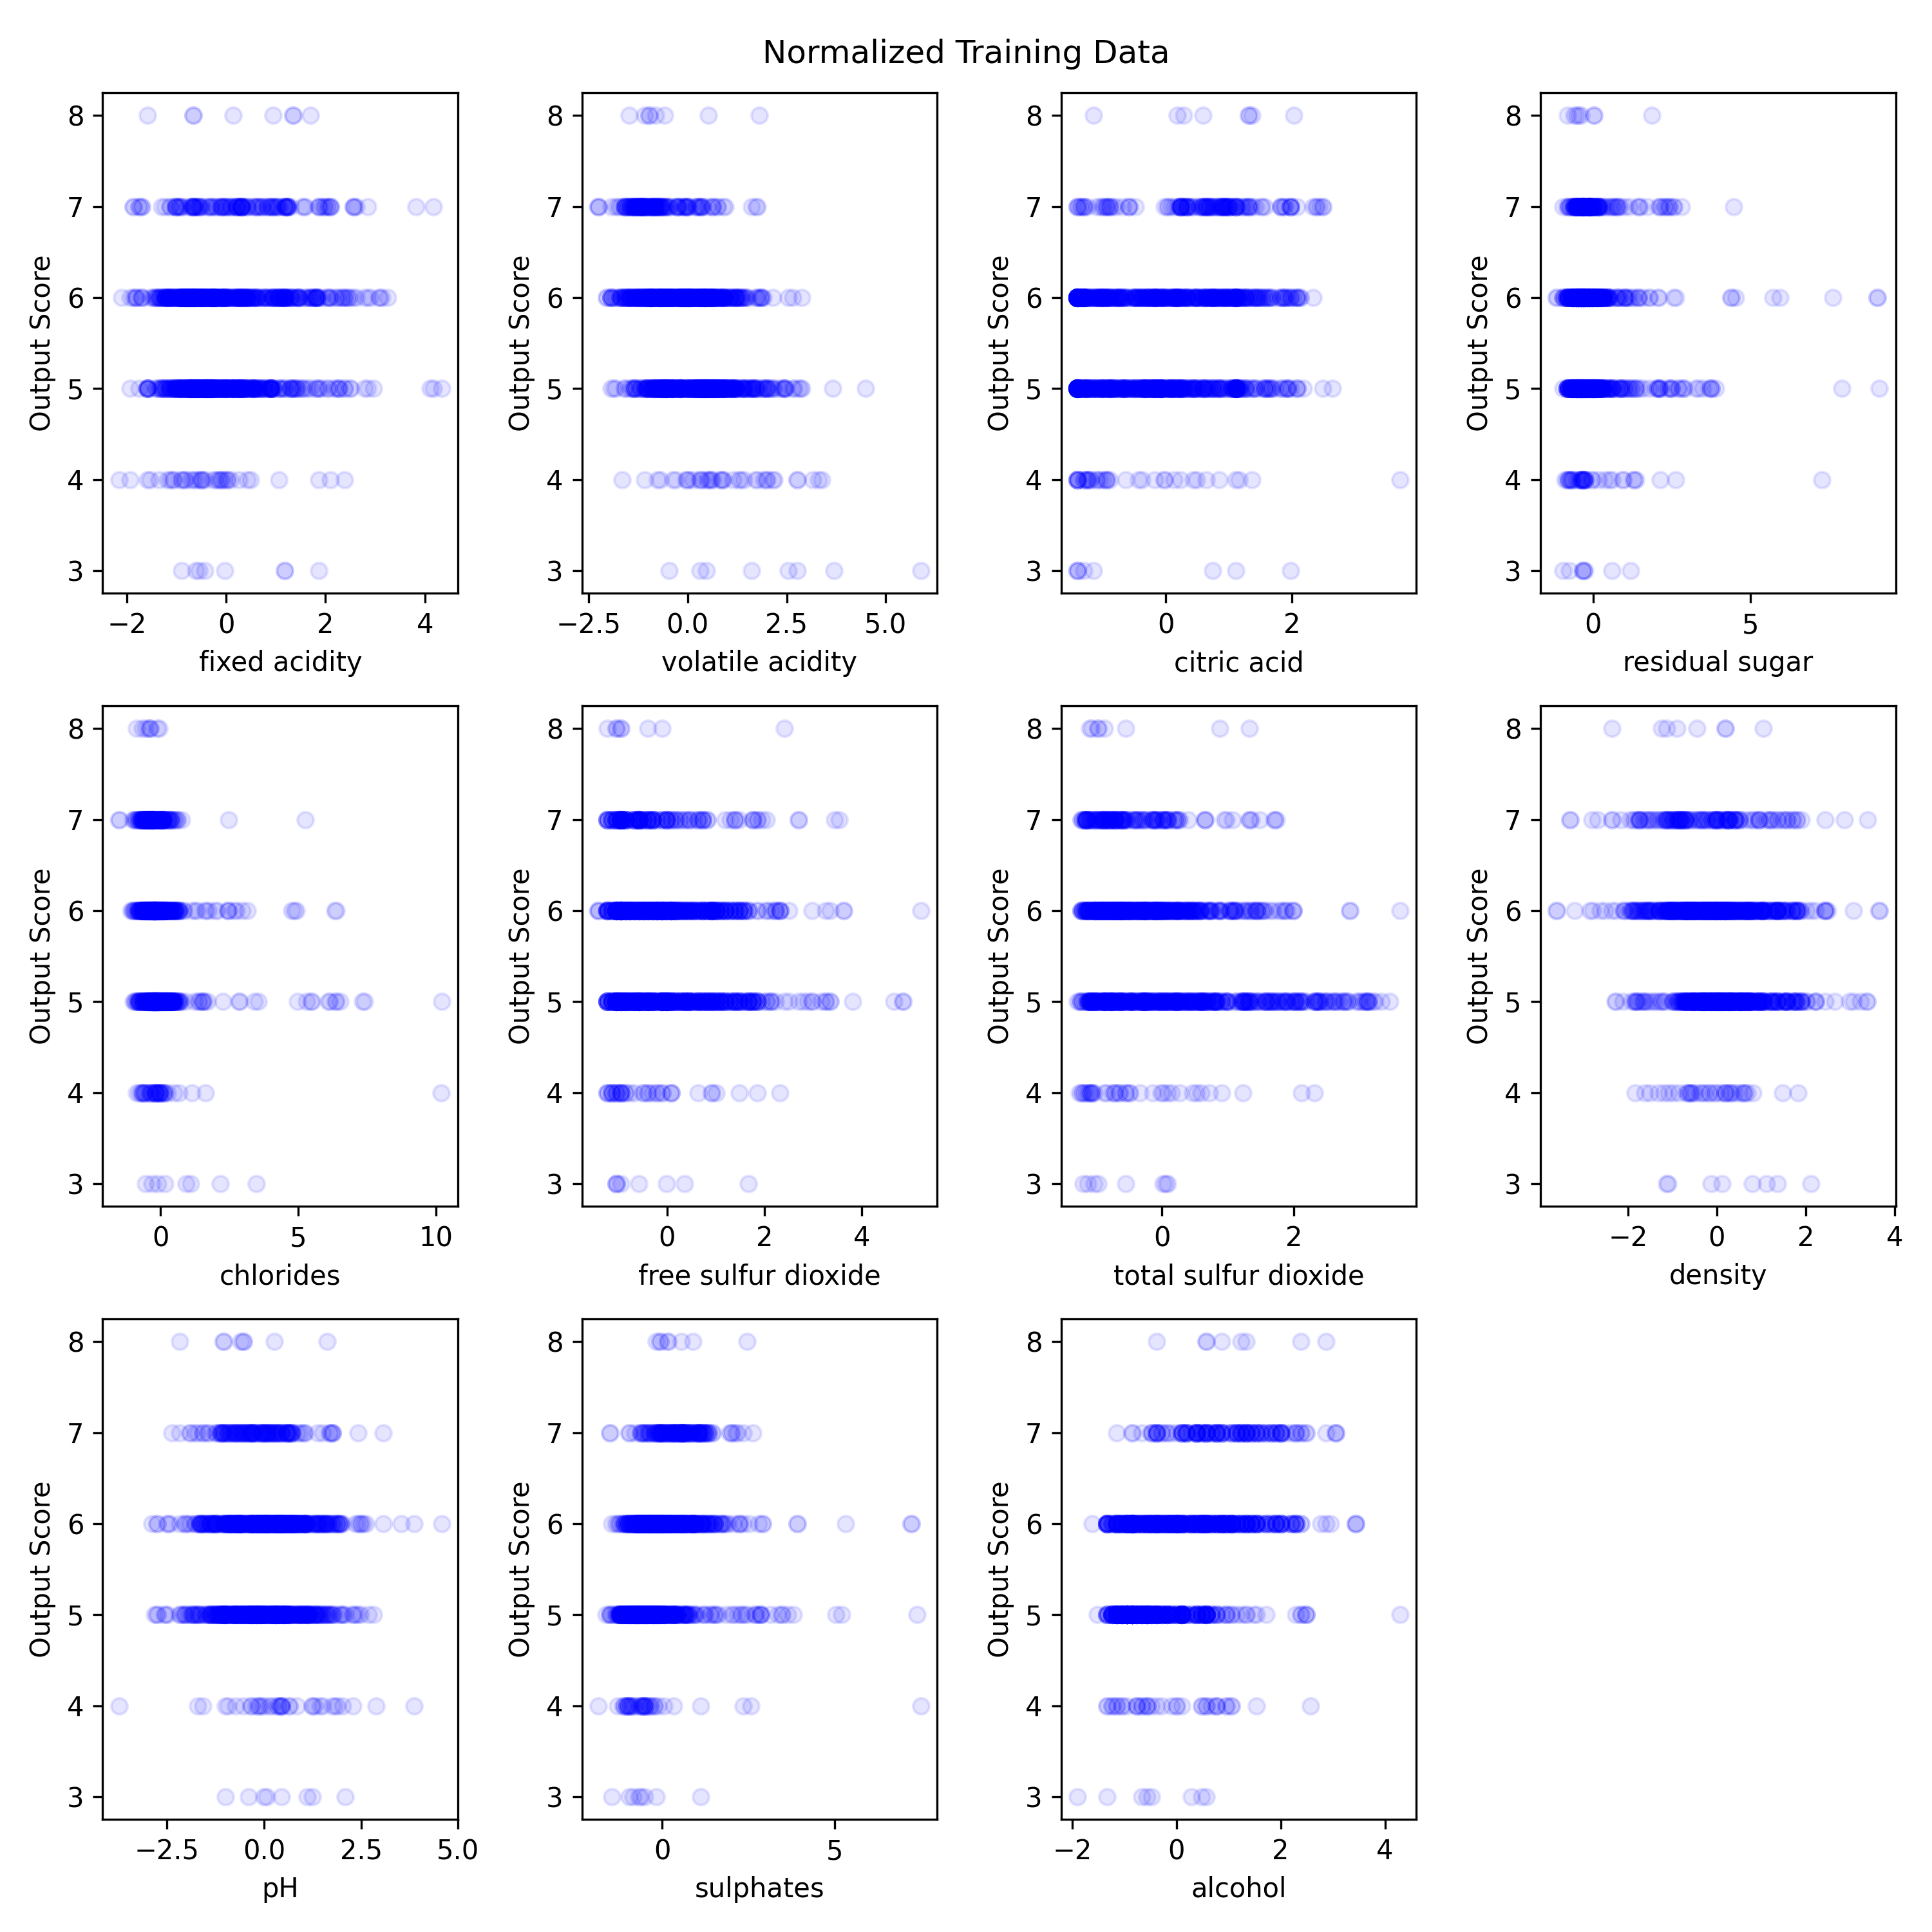
\includegraphics[width=0.8\textwidth]{Figure 1.png}
    \caption{Normalized training data (1115 samples) plotted to show the relationship between any particular 
    chemical feature and the output quality score. Visually, only volatile acidity and alcohol have a clear, linear 
    relationship to the output score.}
    \label{fig:training-data}
\end{figure}

After using linear regression to build a linear model for the training data, the model was evaluated using mean squared error on the 
training data set and on the validation test data set. The linear regression model has a training MSE of 0.494 and a validation MSE of 
o.626. This is a high MSE implying that the model has a limited predictive capacity. Figure \ref{fig:linear-regression-predictions} illustrates 
the limited efficacy of the linear regression model, because it incorrectly predicts that all samples (except one) have an output score 
of 5 or 6.\\

\begin{figure}[H]
    \centering
    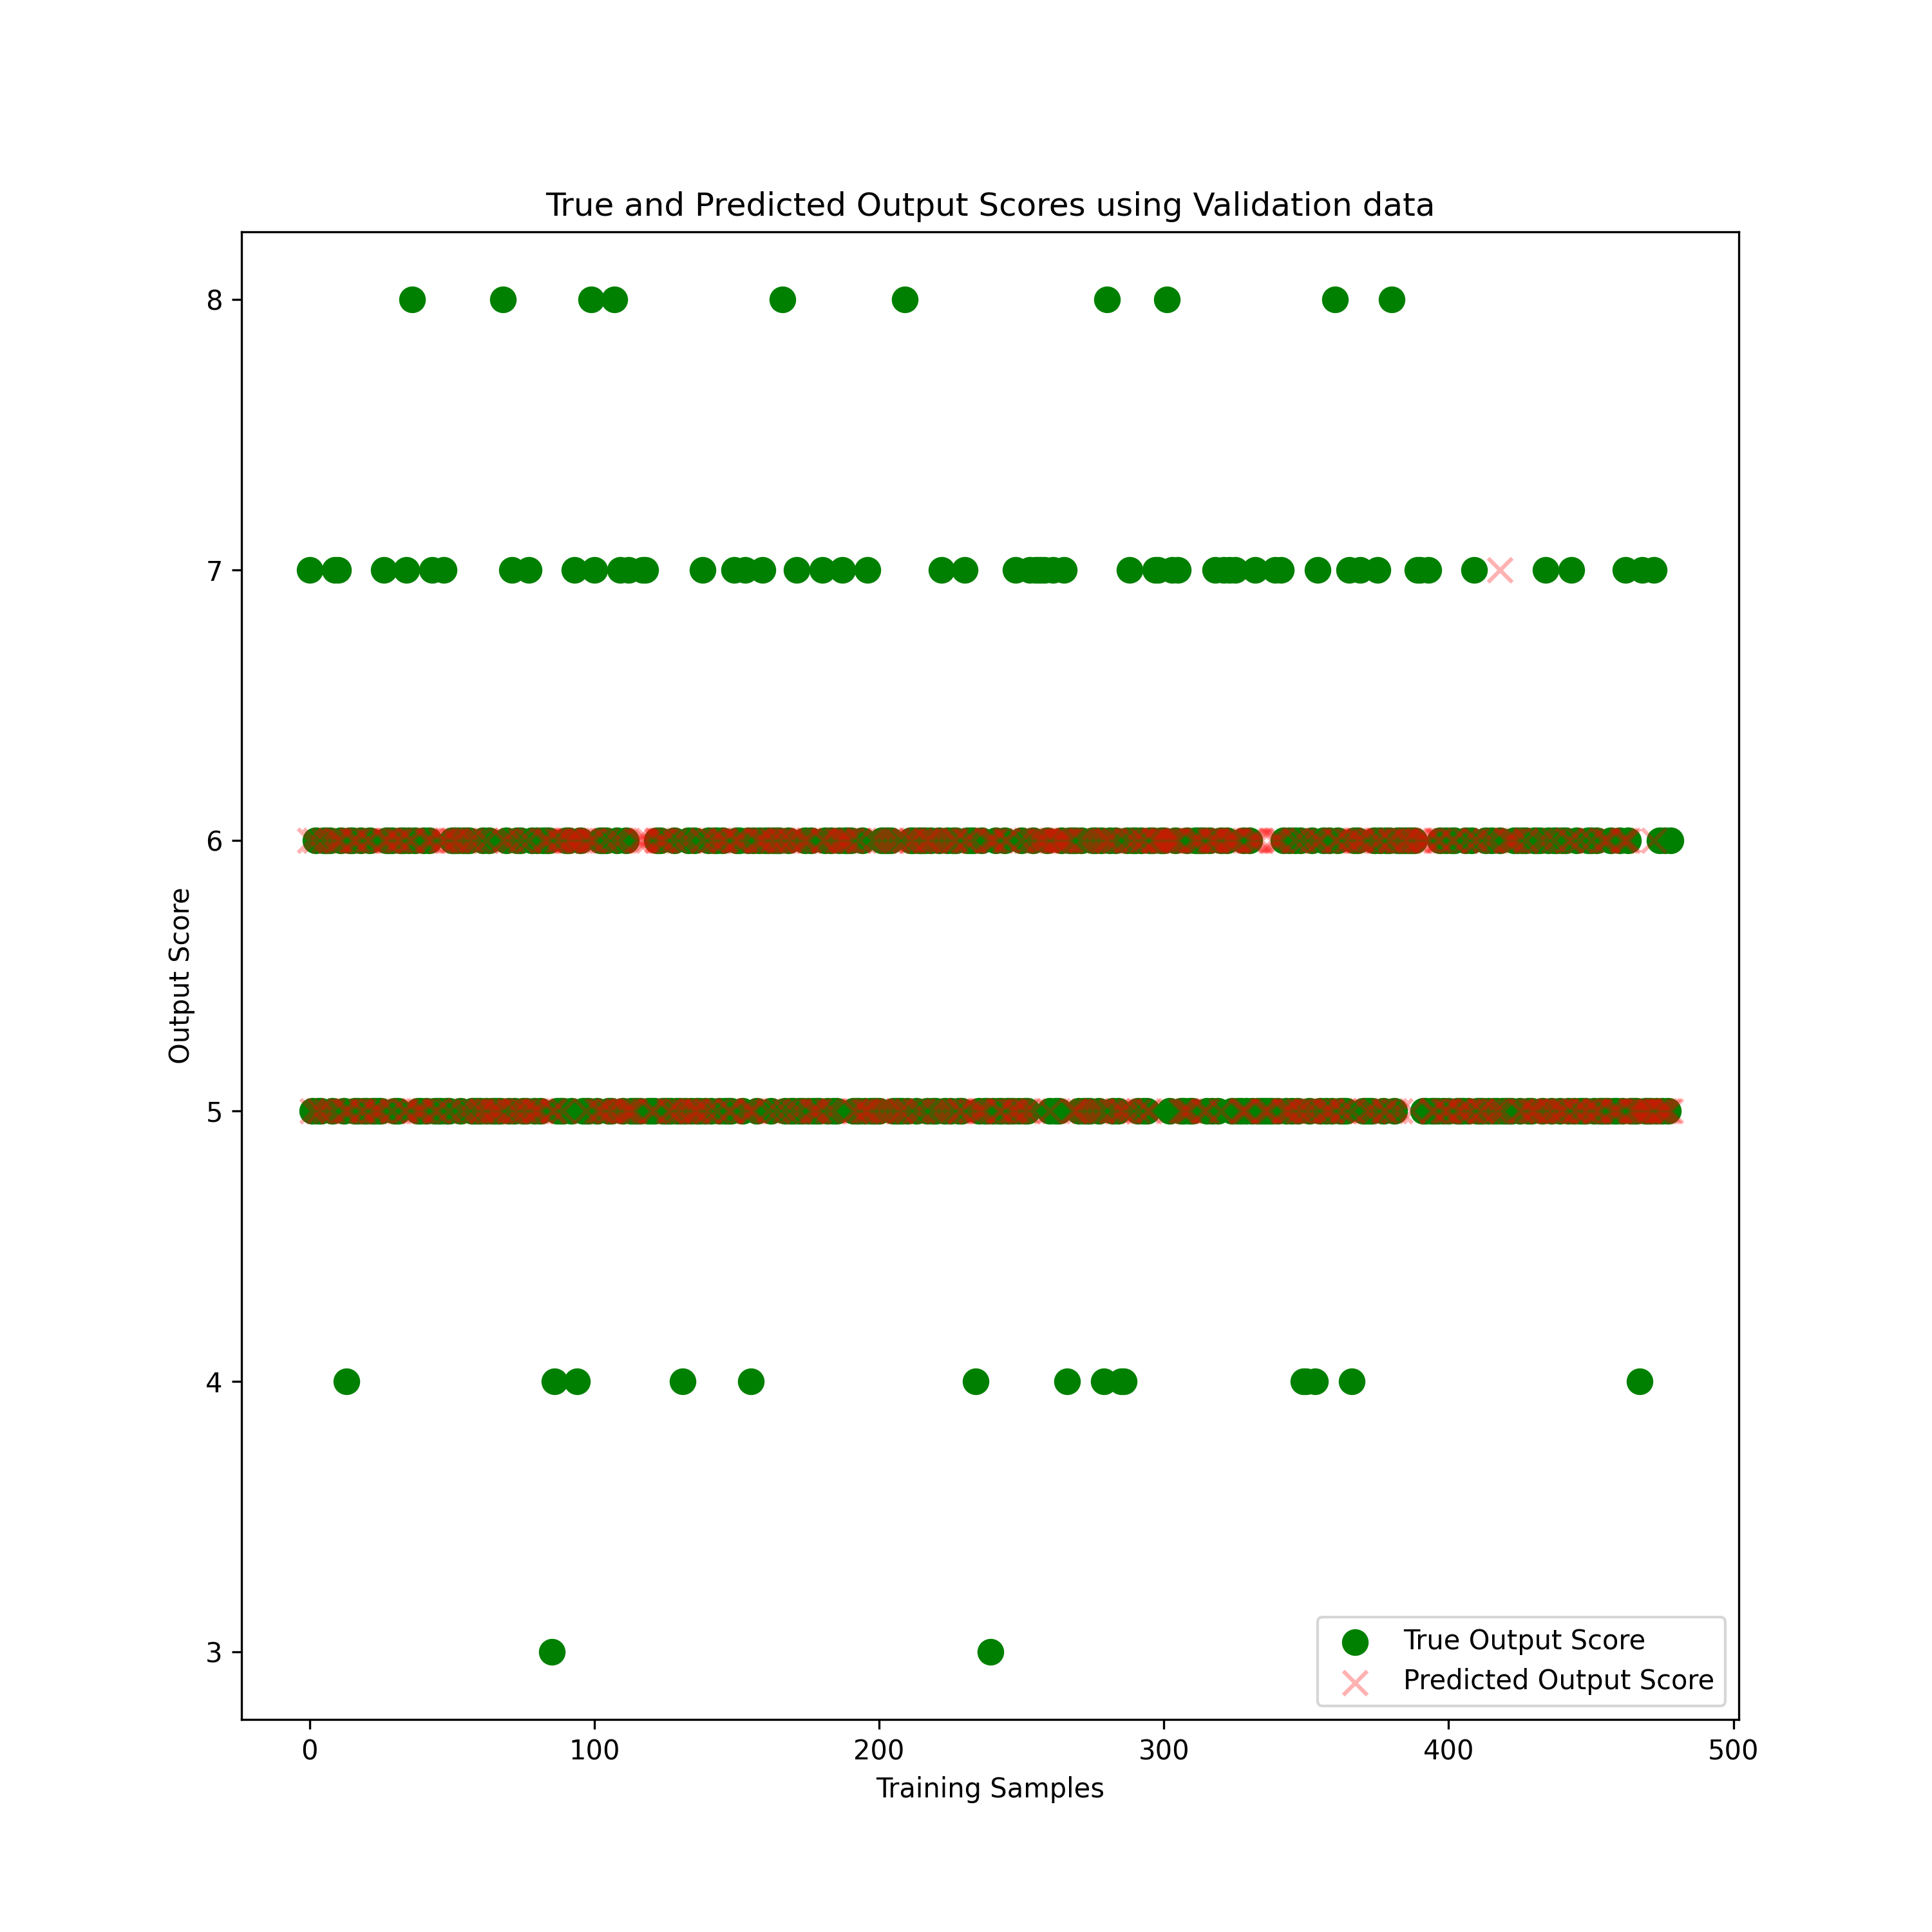
\includegraphics[width=0.8\textwidth]{Figure 2.png}
    \caption{After linear regression was trained on the normalized training data, the model was evaluated against the 
    validation test data (479 samples). The mean squared error is a high 0.626, which is easily seen given the 
    amount of green, 'True' data points that are not overlapped by a red, 'Predicted' data point.}
    \label{fig:linear-regression-predictions}
\end{figure}

Linear models have no artifially introduced degrees of freedom; there is an intercept point ($\theta_0$) and there are 
coefficients ($\theta_i$) for each input feature. We can remove the less meaningful features to reduce modle complexity but 
this will only lower the fitting of the linear model. However, in order to demonstrate this, we wrote a manual ridge regression 
function using the scikit-learn KFold function to calculate how cross validation would impact the training mean squared error by 
increasing the value of $\lambda$ from $10^-1$ to $10^5$. Figure \ref{fig:cv-linear} clearly shows that increasing the value of $\lambda$ 
will only worsen the MSE on the k-folded training data. Therefore, in the linear case, this data is best represented without regularization.\\

\begin{figure}[htbp]
    \centering
    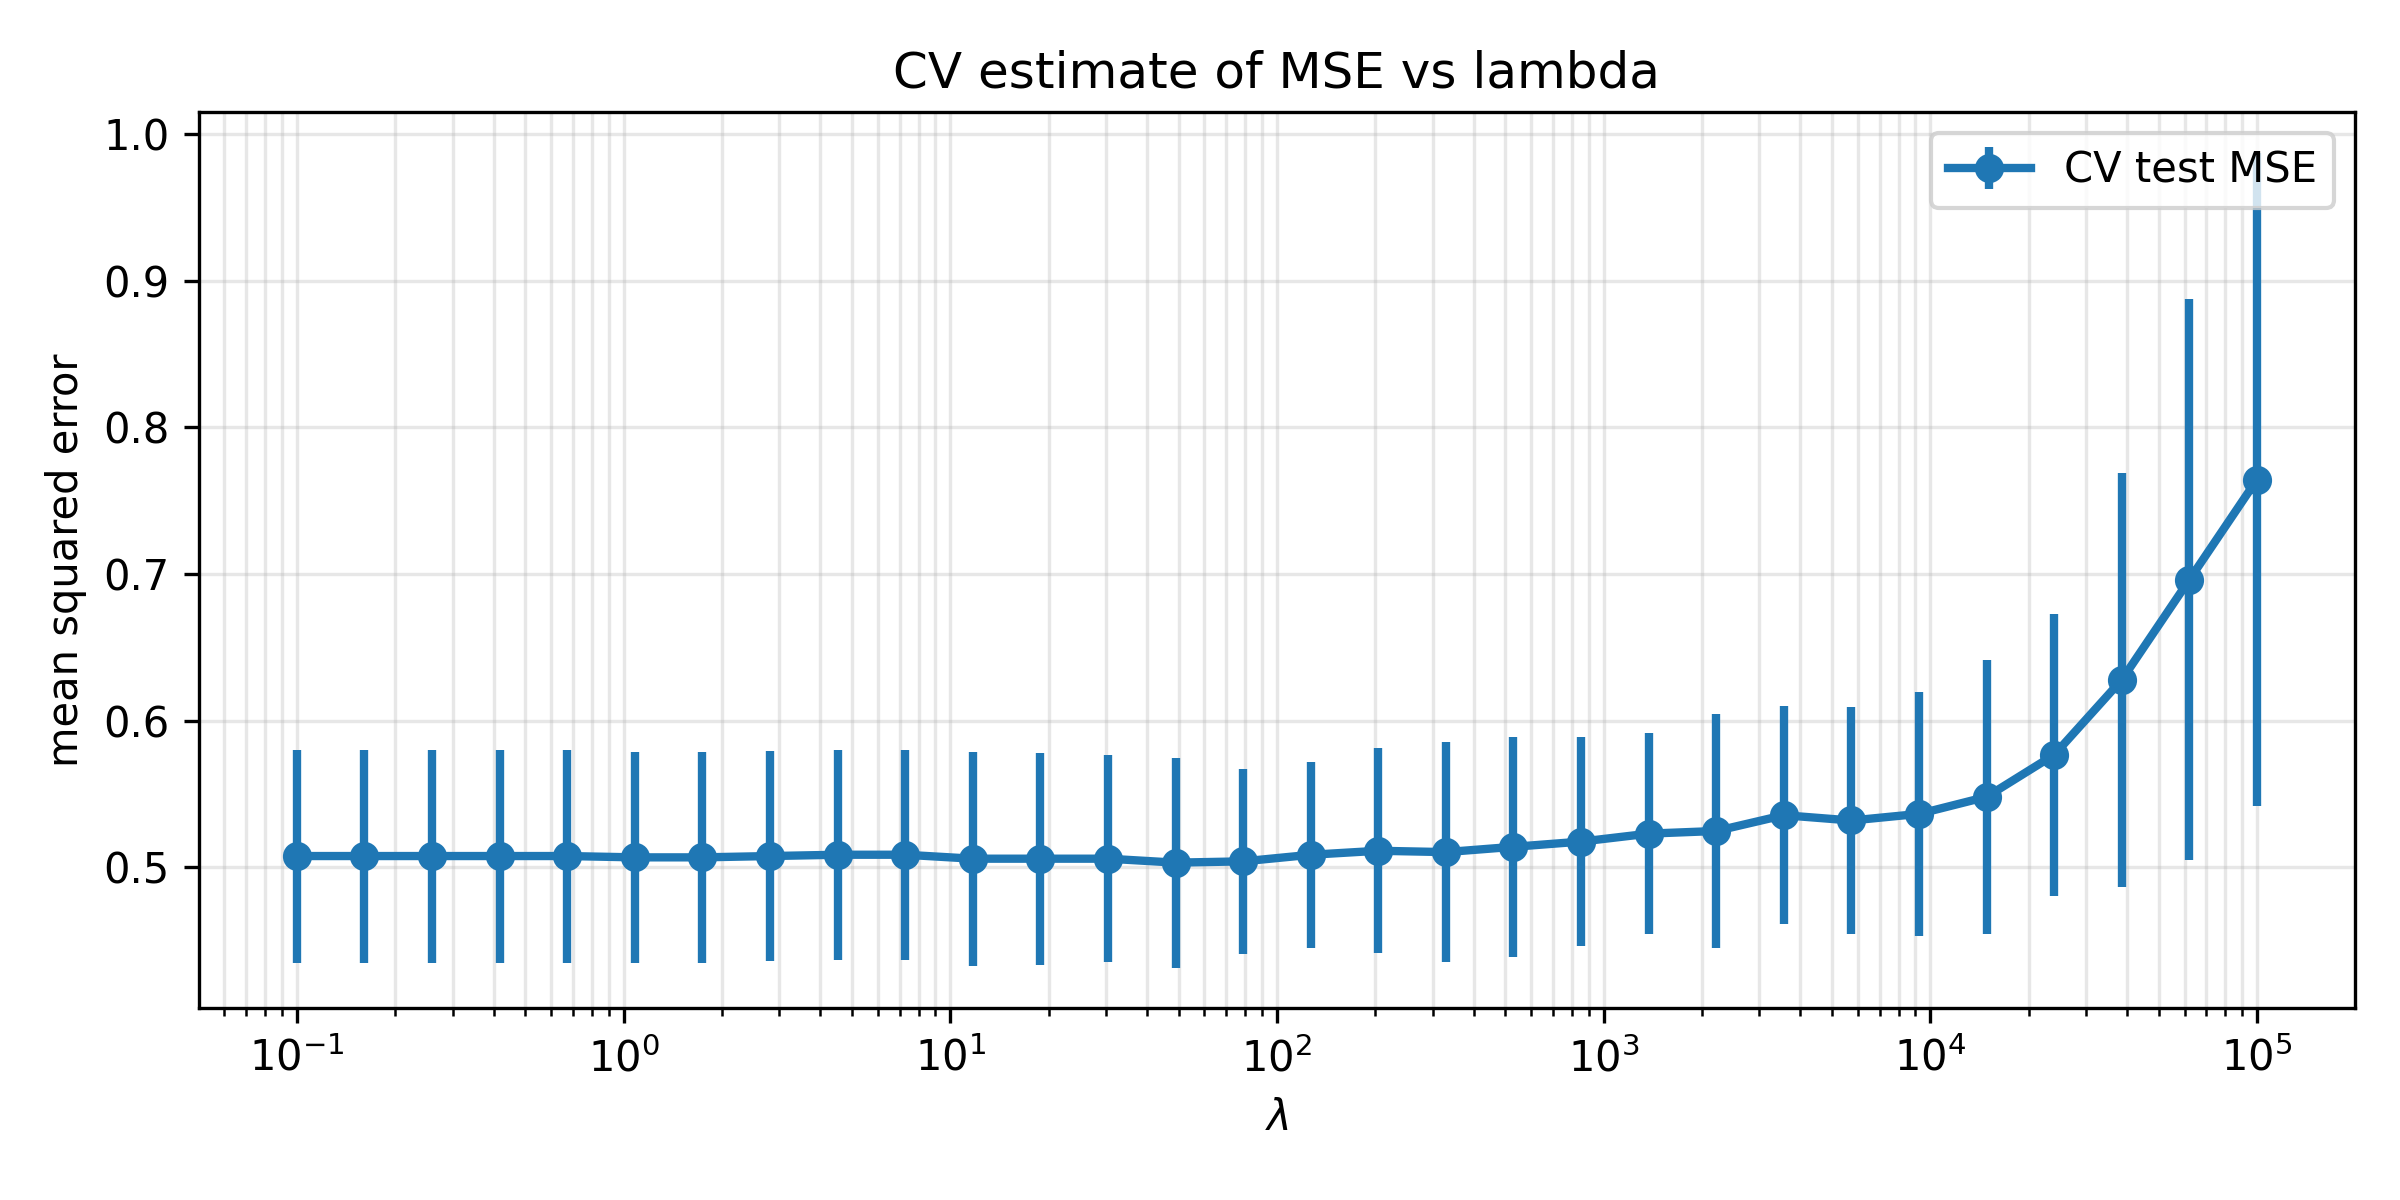
\includegraphics[width=0.7\textwidth]{Figure 3.png}
    \caption{This plot shows that a linear regression model would have the lowest error as it tended towards $\lambda=0$. 
    This was calculated using k-fold cross validation and ridge regression.}
    \label{fig:cv-linear}
\end{figure}

For the Gaussian and Laplacian Kernels, we created a logscale domain of $\lambda$ and $\sigma$ values to opwtimize the model. Then, we 
used the scikit-learn cross val score function to identify the optimal hyperparameters. In the Gaussian kernel, the optimal $\alpha = 1.0$ and $\gamma = 0.125$. 
In the Laplacian kernel, the optimal $\alpha = 0.229$ and $\gamma = 0.198$. This can be seen the \ref{fig:cv-gaussian} and \ref{fig:cv-laplacian} below. We then 
performed a similar cross validation on the Polynomial kernel and found its optimal hyperparameters. In the Polynomial kernel, 
$\alpha = 1.0$, $\gamma = 0.05$, $coef0 = 1$, and $degree = 2$. This points to a polynomial that tended torwards a linear relationship ($degree=2$ and 
$coef0= = 1$) with a low interaction ($\gamma$) between the data points.\\

\begin{figure}[htbp]
    \centering
    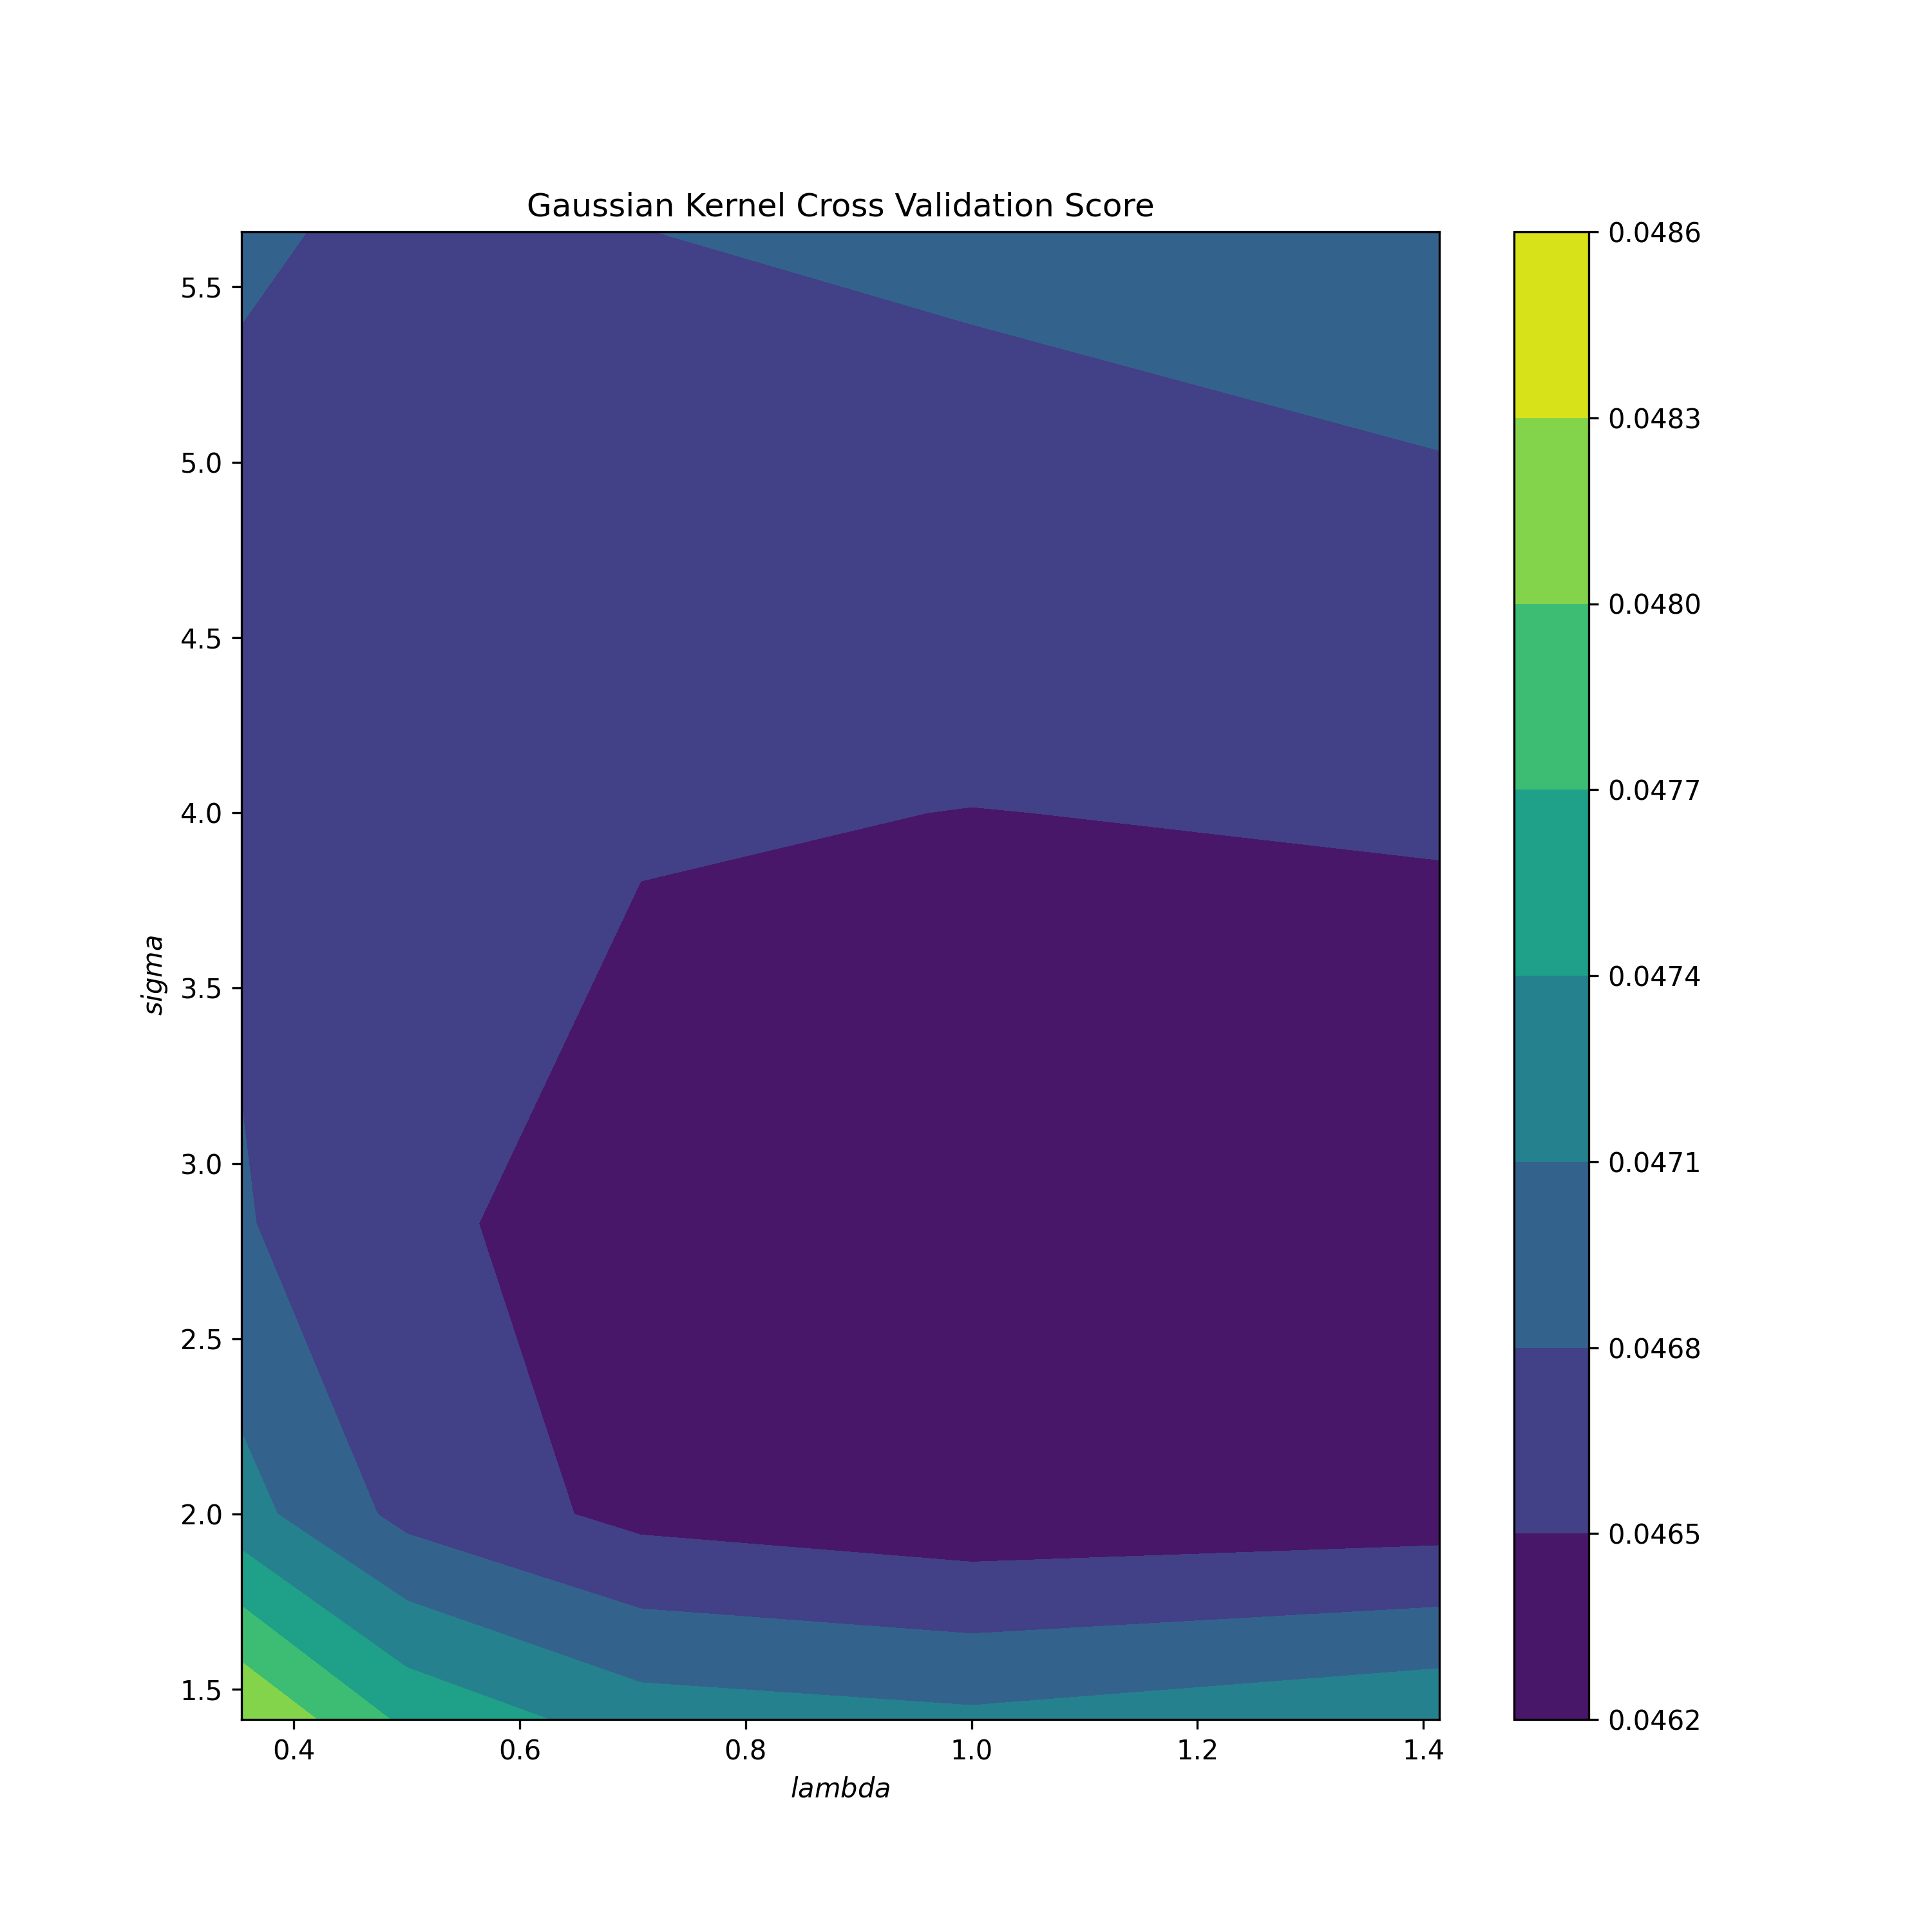
\includegraphics[width=0.7\textwidth]{Figure 4.png}
    \caption{A contour map showing the optimal values of lambda and sigma to reduce error using the gaussian kernel in 
    kernel ridge regression. The optimal parameters are $\lambda=1$ and $\sigma=2$.}
    \label{fig:cv-gaussian}
\end{figure}

\begin{figure}[htbp]
    \centering
    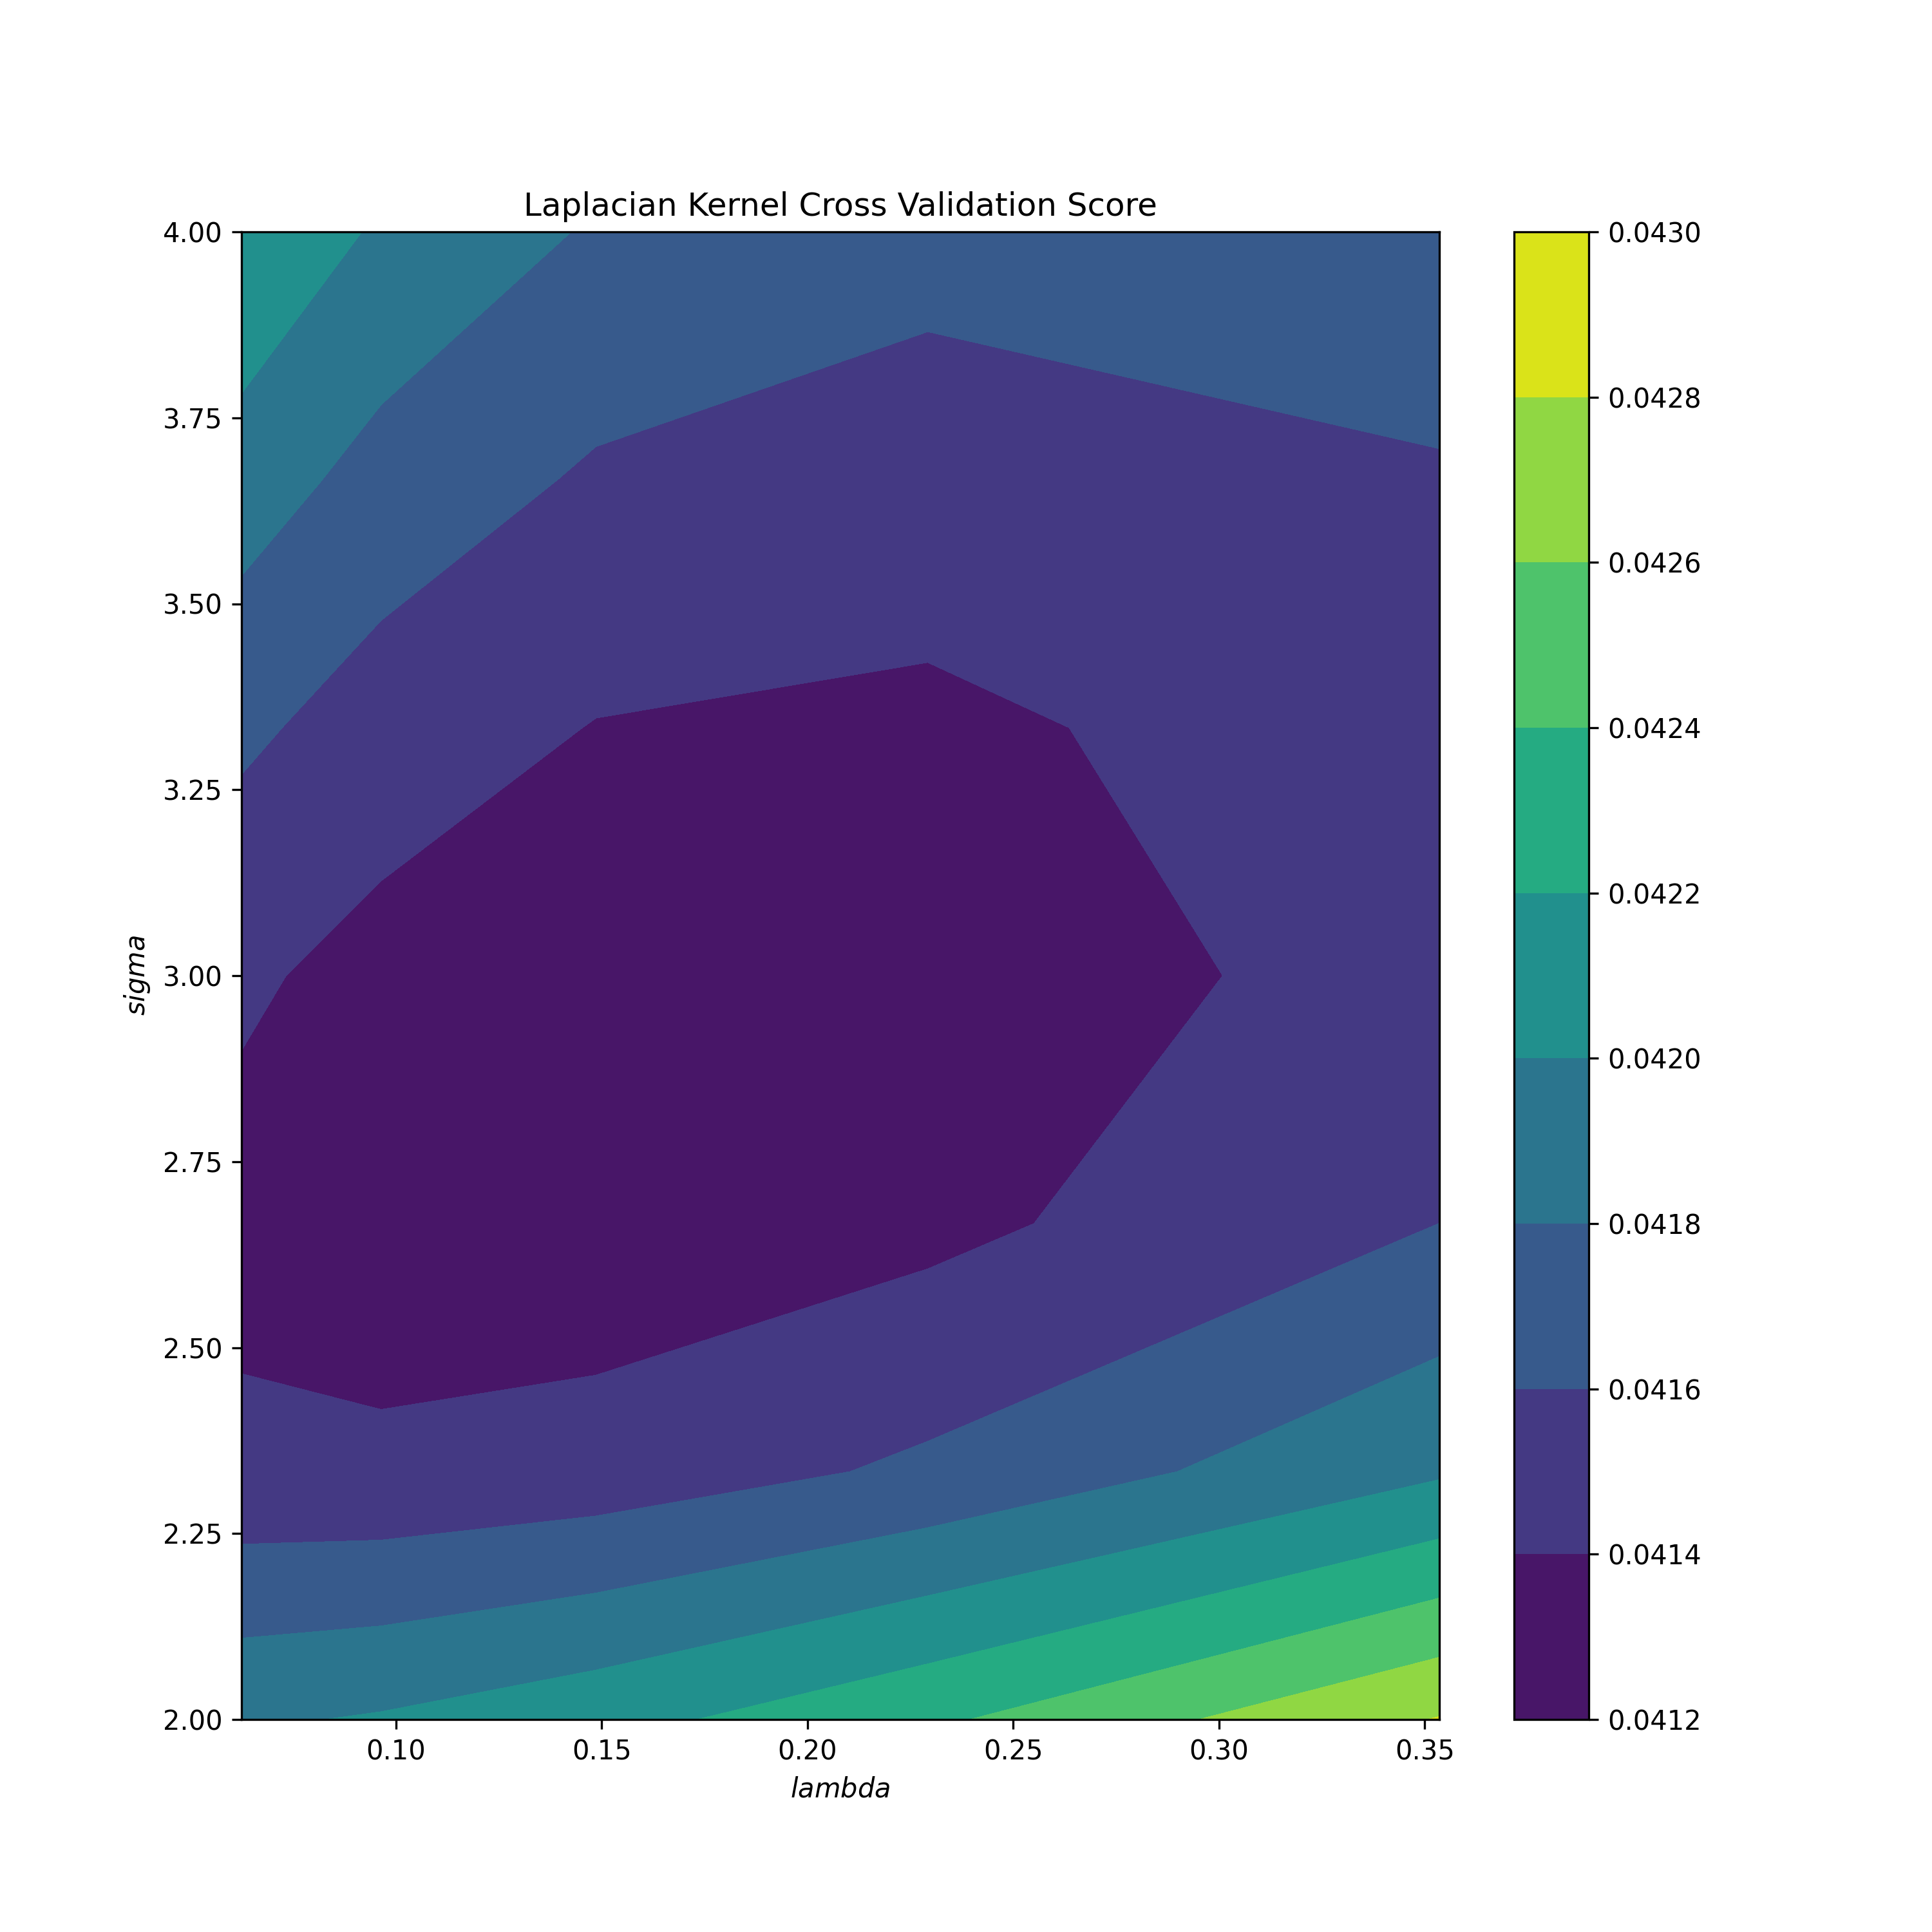
\includegraphics[width=0.7\textwidth]{Figure 5.png}
    \caption{A contour map showing the optimal values of lambda and sigma to reduce error using the laplacian kernel in 
    kernel ridge regression. The optimal parameters are $\lambda=0.230$ and $\sigma=2.333$.}
    \label{fig:cv-laplacian}
\end{figure}

The below two tables show the respective error rates of the four tested models and the output quality scores predicted by the models 
applied to the unknown test data set. The first observation is that none of the models substantially lowered the MSE in the validation test data. 
However, the Gaussian and Laplacian KRR methods were able to lower the training MSE, which suggests that the hyperparameters allowed the model to 
have spurious peaks on the hyperplanes so that the function could 'capture' and correctly classify the known data. The next observation is that 
all four of the models effectively scored the unknown wines the same with small deviations. If we had not used argmax on the output row vectors 
to select the best score, it is fair to assume those vectors would be similar across all four models. Because all four models had a limited range 
of output scores and had such poor MSE scores, it is fair to say that these models fail to display the relationship between these chemical features 
and the wine quality score. 

\begin{table}[H]
    \centering
    \begin{tabular}{|c|c|c|}
        \hline
        Method & Training MSE & Validation MSE \\ \hline
        Linear Regression & 0.494 & 0.626 \\
        Gaussian KRR & 0.299 & 0.564 \\
        Laplacian KRR & 0.299 & 0.564 \\
        Polynomial KRR & 0.449 & 0.541 \\ \hline
    \end{tabular}
    \caption{Side-by-side comparison of the different model classes used as they apply to this data set. The lower MSE scores 
    correspond with a model that can accurately predict the output score based on input features. The validation MSE score is more 
    important as it measures the model's accuracy and precision on information it hasn't seen. However, the high training MSE scores show 
    that these models are largely ineffective.}
    \label{tab:error-table}
\end{table}

\begin{table}[H]
    \centering
    \begin{tabular}{|c|c|c|c|c|c|}
        \hline
        Method & sample 1 & sample 2 & sample 3 & sample 4 & sample 5\\ \hline
        Linear Regression & 6 & 5 & 6 & 6 & 6 \\
        Gaussian KRR & 6 & 5 & 5 & 5 & 6 \\
        Laplacian KRR & 7 & 5 & 6 & 5 & 5 \\
        Polynomial KRR & 6 & 5 & 6 & 6 & 6 \\\hline
    \end{tabular}
    \caption{Output quality scores predicted by the models generated using Linear regression and three variations of Kernal ridge regression.
    applied to the Raw test data.}
    \label{tab:unknown-test-scores}
\end{table}

\section{Summary and Conclusions}\label{sec:conclusions}

Supervised machine learning is an incredibly powerfull tool for classifying information and generating predictions. However, 
these features may not have a causal, or even correlated, relationship with the outputs being measured. Even if the features have 
some relationship, the relationship may be complex with optimal values that are obscured by interactions between those features. 
In this data set, the lowest mean square error on the validation test set was the polynomial kernel ridge regression with an mse = 0.541. 
This is very poor and suggests a need for a deeper or more informed model. Regardless, the four models evaluated here provided similar results 
against the unknown test data.\\

In future iterations, I would do more exploratory data analysis on the individual features and their interactions. I would also try to determine features 
that obfuscated results and would try to limit or remove data that poisons the analysis. 

\section*{Acknowledgements}

I would like to thank Professor Hosseini for his lectures, notes, and code examples.

\bibliographystyle{abbrv}
\bibliography{AMATH_582_HW4_references}

\end{document}
